
\section{What accounts for a successful Cyber Security Strategy?}\label{Sucessful_NCSS}

There are many components, layers and moving parts that needs to be addressed for a successul implementations of a National Information and Cyber Security Strategy.

\begin{itemize}
    \item International standards and policies
    \item Regional standards and policies
    \item National standards and policies
    \item Sector (private or public) policies
    \item Industry standards, best practices and policies
    \item Technical education, proficiencies and comprehentions
    \item Technical solutions and systems implementations
    \item Utilization solutions and enforment of policies
\end{itemize}

Information and Cyber Security is, as with any complex and interconnected systems, only as strong as its weakest link. Requiring all of the components, or layers, listed above to be designed, implemented and function seemlessly together in order to have a solid baseline\footnote[1]{With the emphasis on "baseline", as a 100\% security cannot be achived without implications to other aspects such as usability, interoperability and efficiency. There are trade-offs and comprimises at all levels.} for a National Information and Cyber Security Strategy.

At the very top, and in many cases the starting point of all consequtive items in the list, are the standards and policies defined by the European Union and its individual Member States. A piece of paper, a signed law that starts it all, and mandates action to be taken.

To understand current objectives and standings of Norways Cyber Security Strategy, and its couterparts in the European Union, we need to understand the history behind the strategies itself. The challenges and events that promted for such a strategy. The stakeholders involved, and the policies and regulation derived from the inital effort.

After tracing back the initiative's history and understanding its requirements and objectives. We will be able to understand strategy's current form, the policies derived from it. And the agencies and organizations that was established to implement, monitor and enfoce the strategies. Basically the; who, when, why and how.

\subsection{The European Union's NIS Directive and its Annex}

On the 6th of July 2016, the European Union \footnote[2]{More specifically: the European Comission proposes a Directive, a bill of law, and the EU Council and thhe EU Parliament deliberates and votes if the new Directive or bill will pass, be approved.} has approved and signed off on \acrfull{nis}. It is a legislation affecting all European Union member states, and its trading partners in the \Gls{ESM} \footnote[3]{\url{https://en.wikipedia.org/wiki/European_Single_Market for moredetails}}. All EU Member States are mandated to "tranpose", or incorporate the directive into their National legislations and have a \acrfull{ncss} by 9th of May 2018.

The Directive has 3 annex documents. The annexies provides more context and clarity to the Directive. Where the Directive can be regarded a as formal legislative document, with the language to match. The annex documents explains and expands on the task, requirements and scope of the Directive with a language that matches its intended audience.

\begin{itemize}
    \item Annex 1
        \begin{itemize}
            \item Provides guidance to the tasks and clarification of the requirements pertaining to the NIS Directive.
        \end{itemize}    
    \item Annex 2
        \begin{itemize}
            \item Identifies the sectors and subsectors considered as higly critical in provisioning the services for each Member State and the Union as a whole.
        \end{itemize}
    \item Annex 3
        \begin{itemize}
            \item Outlines the services regarded to essential for the functioning the population for each Member State and the Union as a whole.
        \end{itemize}
\end{itemize}

In the 2nd of October 2020, a review of the Directive has been conducted, and a revised NIS has been presented and proposed to the European Comission on 6th of December 2020 by the NIS Cooperation Group.

\subsubsection{NIS' objectives}
According the the NIS Corrigendum, \cite{EuropeanCommission2017} , a communication by the European Commission to its Member States, the Directive has 3 main objectives:

\begin{itemize}
    \item Improving nationanl cyber security capabilities,
    \item Building cooperation at EU level, and
    \item Promoting a culture of risk management and incident reporting among key economic actors, notably \acrfull{oes} for the maintenance of economic and scietal activities and \acrfull{dsp}.
\end{itemize}

However, each Member State are expected to expand on the 3 main objectives, and define its \acrshort{ncss} according to each Member State's specific needs and priorities as long as it is never below the requirements and objectives set in the NIS Directive.

\subsubsection{NIS' scope}

As indicated in the list above, Annex 2 and 3 outlines the scope of the directive. The Directive does not describe in detail what the scope is. Instead the Annex provides a guideline to identify what constitutes a \acrfull{oes}, as can be read in Section 4.1 in the Annex 3 \acrshort{oes}. As of 16th of December 2020, NIS2\footnote[4]{Please see more details regarding NIS2 in \url{https://ec.europa.eu/digital-single-market/en/news/revised-directive-security-network-and-information-systems-nis2}} proposal has been sent to the European Comission expanding the scope of sectors and services from 7 to 15. 

\begin{figure}[H]
    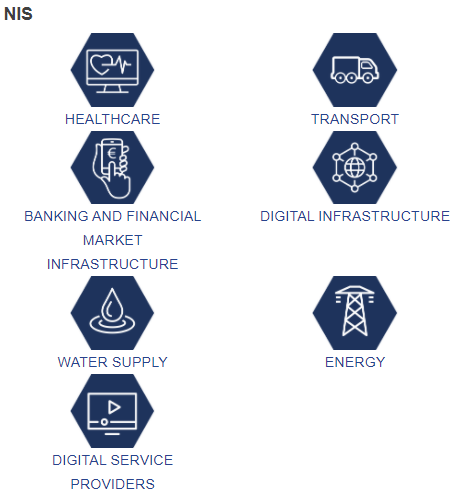
\includegraphics[width=0.4\textwidth]{tex/NIS1_Sectors_and_Scope.png}
\end{figure}
\begin{figure}[H]
    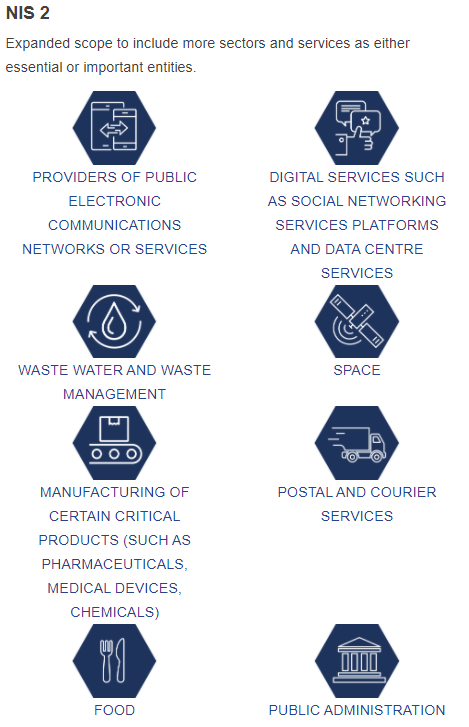
\includegraphics[width=0.4\textwidth]{tex/NIS2_Sectors_and_Scope.png}
\end{figure}

With regards to the Banking and Financial Sector, NIS directive requires that member states that are not within the Banking Union to be regulated and supervised by a relevant banking authority. Such is the case for Norway, by having Finans Tilsynet as the Financial Authority with the responsibility to enforce policies for security measures and mandate standards as required within the European Union or by the different banking, exchange and securities \footnote[5]{Security as a financial term: a tradable financial assesset. Not security as adjective for safety, or verb as to "secure something".} authorities and agencies.

\subsubsection{The NIS Trasposition}

Looking back at the list, the layered components of a Cyber Security Strategy from page \pageref{Successful_NCSS}, the transposition of the NIS Directive is the adoptation of the Directive into each Member States national standards and policies for Information and Cyber SEcurity. The NIS Deirective has set the deadline for its Member States to have conducted the trasposition by 9th of May 2018.

The EU Commission is aware of the challenges with regars to the transposition of the Directive into each Members State's legislationThe adoptation of the Directive does not require a full impl


\subsubsection{Review and continuos improvement}

The European Commission actively monitors and assesses each of its members states adaptation and implementation of the NIS Directive. The European Commission official website\footnote[3]{\url{https://ec.europa.eu/digital-single-market/en/state-play-transposition-nis-directive}} provides a tool and an interactive map to navigate and view each members states current implementation of the strategy, the agencies and authorities involved as well as each Member State's \acrshort{ncss}.

Furthermore, the NIS directive §4 outlines the importance of having all the members of the European Union engages with the issues involving Cyber Security collectively. Having a cross border collaboration and sharing of information are key to defeating a threat that is inherently agnostic to geographical location and legal jurisdiction, NIS §6. \cite{VIIRA2018} 

The provisions regarding collaboration, sharing of information and close monitoring and assessement of the policies implemented provides the Commission and all Member States a very good foundation to evaluate and improve the NIS Directive.


\subsection{Cyber Security Stakeholders in the European Union}

There certain requirements described in the NIS that every member states must comply with. Amongst are the requirement to establist certain egancies to manange and monitor the directives and strategies and to enforce the policies derived from it. One such agency is the establishment of National \acrfull{csirt}


\begin{followup}
    Outline the entities, their roles and responsibilities with regards to the OES, CIIP and the Finance sector:
    \begin{itemize}
        \item NIS Cooperation Group (\url{https://ec.europa.eu/digital-single-market/en/nis-cooperation-group})
        \item ENISA
        \item The European System of Financial Supervision - Sectore regulation and supervision.
        \item The European Securities Markets Authority - Direct supoervision of credit-rating agencies and trade repositories
    \end{itemize}

    How lex specialis applies with NIS and Norways National laws and regulations.
\end{followup}


\begin{followup}
    Remember to put link to section "Legislation process"
    Describe the difference between Decision, Directive and Regulation
\end{followup}

 Online archive of European Union Law: \url{https://eur-lex.europa.eu/homepage.html?locale=en}

\newpage

\subsection{The Norwegian National Cyber Security Strategy}

Norways approach to its \acrshort{ncss} is largely in compliance with the NIS Directive. Although Norway is not directly mandated to adhere to the NIS Directive, aligning and being compliant with EU's regulations and policies is both sensible and benefitial. 

Finance sector regulations, Communications and Privacy laws are a couple of example that benefits Norway by allowing for free movement of goods, persons, services and capital with other\acrshort{eea} Member States. Compliance and with the mentioned laws and regulation makes it much simplier by implmenting \acrshort{ncss} in accordance with the NIS directive.

\subsection{Establishing Norways NCSS}

\begin{followup}
    Outline the processes and committes involved establishing the strategy:

    The Ministry of Justice and Public Security is
    responsible for the preservation and development
    of basic guarantees of the rule of law.

    **Definition**
    NOU = Norges offentlige utredninger
    by \url{https://snl.no/Norges_offentlige_utredninger_(NOU)} Norges Store Leksikon

    **The Process**
    - A government or any of its departments recognizes a problem-area,
    an issue, and is set on a task to remediate for the country's
    electorate and society at large.

    - The department entity then establishes a committee, a council,
    whom are designated a mandate and an objective to work on the case.

    - The committee can be comprised of many different entities. Both
    public, private or ideal organizations. Researchers, subject matter
    experts or anyone who may provide valuable contributution to the
    endevour.

    - The committee is tasked to investigate and report their findings
    back to the responsible/sponsor government department.

    - The findings are subject further for debate and political process
    by the departments, public or private organizations or other
    stakeholders and interested parties.

    - The process will decide if there is merit for the findings to
    be submitted and presented to the parliament for legislative process.
    The findings are presented as a white paper, a Stortingsmelding,
    which will be a 
end note

Stortingsmelding/White Paper

    \url{https://www.regjeringen.no/no/dep/jd/org/styre-rad-og-utval/innstillinger/innstillinger-fra-utvalg/innstillinger-levert-i-2018/IKT-sikkerhetsutvalget/id2570775/}
    
    IKT-sikkerhetsutvalget
    Skattedirektør Hans Christian Holte, Oslo (leder)
    Direktør - Cybersikkerhet Terje Wold, Tromsø
    Administrerende direktør Håkon Grimstad, Trondheim
    Head of Information Security Lillian Røstad, Nesodden
    Direktør internett og nye medier Torgeir A. Waterhouse, Oslo
    Forskningsleder Marie Moe, Trondheim
    Professor Lee A. Bygrave, Oslo
    Lagdommer Therese Steen, Oslo

    The Committee established a reference group and consult with
    stakeholders from different ministries and departments:
    - Minister of Justice and Public Security - Monica Mæland (Conservative Party)
    - Ministry of Defence - Frank Bakke-Jensen (Conservative Party)
    - Ministry of Local Government and Modernisation - Nikolai Astrup (Conservative Party) Linda Hofstad Helleland (Conservative Party)
    - Ministry of Transport - Knut Arild Hareide (Christian Democratic Party)
    - Ministry of Trade, Industry and Fisheries - Iselin Nybø (Liberal Party) Odd Emil Ingebrigtsen (Conservative Party)
    - Office of the Prime Minister - Erna Solberg (Conservative Party)
    - Nasjonalt cybersikkerhetssenter

    The committees effort has its foundation from:
    - \url{https://www.regjeringen.no/no/dokumenter/nou-2015-13/id2464370/} NOU 2015: 13 Digital sårbarhet – sikkert samfunn ble våre digitale sårbarheter kartlagt
    - \url{https://www.regjeringen.no/no/dokumenter/meld.-st.-10-20162017/id2523238/} Meld]]. St. 10 (2016–2017) om samfunnssikkerhet
    - \url{ttps://www.regjeringen.no/no/dokumenter/meld.-st.-38-20162017/id2555996/} Meld]]. St. 38 (2016–2017) IKT-sikkerhet — Et felles ansvar

    The committee must adhere to:
    - Prop. 153 L (2016 – 2017) \url{https://www.regjeringen.no/no/dokumenter/prop.-153-l-2016-2017/id2556988/} Lov om nasjonal sikkerhet]]
    -- Proposal from the Ministry of Defense based on a NOU from 2016: 19
    - Personvernregelverk / Privacy law
    - GDPR


    The committee's deliverable was a white paper \url{https://www.regjeringen.no/no/dokumenter/nou-2018-14/id2621037/} NOU 2018: 14 IKT-sikkerhet i alle ledd — Organisering og regulering av nasjonal IKT-sikkerhet, white paper
    addressing 3 key issues (released on 2018-12-03):
    1) Applicability and aptness
    2) Organization and coordination
    3) According to findings in 1 and 2, establish and enforce
    effective regulations following EU NIS Directive.

    The \url{https://www.regjeringen.no/no/aktuelt/utvalg-foreslar-flere-tiltak-for-en-sterkere-nasjonal-ikt-sikkerhet/id2621146/} press release from IKT Committee concludes:
    Norway's Information and Communication Technology Security
    was inadequately legislated and regulated.

    The report outlined the need for a law to be passed for
    Governmental Procurement and acquisitions where
    ICT Security is relevant.
    
    New laws and regulation must be establish to regulate
    ICT Security where Public Services and Critial Information
    and Communication Infrastructure can be impacted.

    A centralized national ICT Security organization is
    proposed to be established. An organization who can
    operate horizontally between state departments, agencies
    and private entities. Who's responsibility is to manage
    and coordinate Norway's ICT Security effort.
\end{followup}


\subsubsection{Norways Objectives}

\begin{followup}
    Expand and elaborate on:

    National Cyber Security Strategy

        **Vision**
        In Norway, it is safe to use digital services. Private
        individuals and companies have confidence in national
        security, and trust that the welfare and democratic rights
        of the individual are being safeguarded in a digitalised
        society.

        **Strategic Goals**
        1. Norwegian companies digitalise in a secure and
        trustworthy manner, and are able to protect themselves
        against cyber incidents

        2. Critical societal functions are supported by a robust and
        reliable digital infrastructure
        
        3. Improved cyber security competence is aligned with the
        needs of society
        
        4. Society has improved ability to detect and handle cyber
        attacks
        
        5. The police have strengthened their ability to prevent
        and combat cyber crime
\end{followup}


\subsubsection{Norways Objectives}

\begin{followup}
    Refer to the BDO analysis that compares Norways strategy with EU's Directive. Ref \url{https://www.regjeringen.no/contentassets/fe88e9ea8a354bd1b63bc0022469f644/no/sved/1.pdf}. An Analysis performed by BDO which cover the objective of this project.

    Instead of redoing and performing the anaylisis again. Refer to the findings and recommendation from the BDO analysis in combination with the EU's own NIS analysis. And perform a meta anaylisis on both.
\end{followup}